% This is LLNCS.DOC the documentation file of
% the LaTeX2e class from Springer-Verlag
% for Lecture Notes in Computer Science, version 2.4
\documentclass{acm_proc_article-sp}

\usepackage{color}
\usepackage{graphicx}
\usepackage{listings, tikz, xcolor}
\usepackage{bold-extra}
\usepackage{subfig}
\usepackage{enumerate}
\usepackage[backgroundcolor=pink!40, disable]{todonotes}
\usepackage{courier}
\usepackage{syntax}
\usepackage{amsmath}
\usepackage{amsthm}
\usepackage{hyperref}
\usepackage{MnSymbol}

\definecolor{lightGrey}{rgb}{0.9, 0.9, 0.9}
\newcommand{\hilight}{\makebox[0pt][l]{\color{lightGrey}\rule[-0.45em]{0.9\linewidth}{1.5em}}}
\newtheorem{mydef}{Definition}
\DeclareCaptionType{copyrightbox}
%
\lstset{ 
	language = [AspectJ]Java,
  basicstyle=\sffamily\small,
  numbers=left,
	numberstyle=\tiny\color[rgb]{0.25,0.25,0.25},
	numberblanklines=false,
  firstnumber=auto,
	breaklines=true,
  tabsize=2,
	emph={aspect,declare, adapter, instance, pointcut, adaptee, adapts, select, UNTIL,pc, instanceType, exp, removeExp, subsetof, supersetof}, 
	emphstyle=\textbf,
	escapechar={~},
	showstringspaces= false,
	frame=single,
	captionpos = b,
	numberbychapter=false,
	breakatwhitespace = true,
	columns=fullflexible
	}
\lstset{prebreak=\raisebox{0ex}[0ex][0ex]{\ensuremath{\rhookswarrow}}} % requires \usepackage{MnSymbol}
%\lstset{postbreak=\raisebox{0ex}[0ex][0ex]{\ensuremath{\rcurvearrowse\space}}} % requires \usepackage{MnSymbol}	
	
\usetikzlibrary{arrows,shapes.multipart,shapes.arrows,shapes.misc,calc,fit,shadows,positioning,patterns} 

\newcommand\bh{\tikz[remember picture]
					\node (begin highlight) {};
			 }
  \newcommand\eh{\tikz[remember picture]
		 \node (end highlight) {};
		 \tikz[remember picture, overlay] 
		 \draw[yellow,line width=10pt,opacity=0.3] (begin highlight) -- (end
			highlight);
		 }

\newcommand{\lstinlineabstract}[1]{\lstinline[emph={#1},emphstyle=\textit]{#1}}
\begin{document}


\title{Instance Pointcuts:}
\subtitle{An Aspect-Oriented Mechanism for Maintaining Object Categories}

\numberofauthors{1}
\author{
\alignauthor
Kardelen Hatun \hspace{2cm} Christoph Bockisch \hspace{2cm} Mehmet Ak\c{s}it\\
\affaddr{TRESE, University of Twente, 7500AE Enschede, The Netherlands}\\
\affaddr{\url{http://www.utwente.nl/ewi/trese/}}\\
\email{ \{hatunk,c.m.bockisch,aksit\}@ewi.utwente.nl}
}


\maketitle

\begin{abstract}
In the life-cycle of objects there are different phases. The phase in which an object currently is, affects how it is handled in an application; however these phase shifts are typically implicit.
In this study we propose an extension to the aspect-oriented language AspectJ with a new mechanism, called instance pointcuts, for categorizing objects according to events in their life-cycle; these events are selected with pointcut-like specifications.
The selection criteria of instance pointcuts can be refined, e.g., to define a subset or super-set of an existing instance pointcut; and they can be composed, e.g., by set operations.
We offer a means to access all objects currently selected by an instance pointcut from Java code, i.e., to be used in methods or advice bodies; and we expose the events of adding a or removing an object from an instance pointcut by creating a join point that can be selected by regular pointcuts.
Our approach improves modularity by providing a fine-grained mechanism and a declarative syntax to maintain a set of objects.
\end{abstract}

\section{Introduction}
In object-oriented programming (OOP), objects encapsulate state and behavior; objects also have a life-cycle, which means that the same object can play different roles at different times.
And which role an object is currently playing can affect the object's own behavior or how it is handled.
Typically the shift from one life-cycle phase to another is implicit marked by events, e.g., when by passing an object from one client to another.
Aspect-oriented programming (AOP) is a well-known technique for modularly implementing behavior applicable at events emitted from code that is not localized in a single type hierarchy.
But current aspect-oriented languages do not offer declarative abstractions of object sets based on other criteria then the type, which is basically the same as plain object-oriented languages.
In this paper, we propose a new language mechanism for declaratively specifying life-cycle phases and for exposing the set of objects which are currently in a specific phase. This declarativity allows us to give guarantees about these sets like subset relationships, as well as to perform compile-time checks like warning about sets that will always be empty. \textbf{Do we discuss checks?}

As an example of different relevant phases in the life-cycle of objects, consider an online store application with ``customer'' objects representing the purchasers and ``item'' objects representing the products they add to their ``shopping-bags''. We want to add discount policies for products that are treated by the customers in specific ways: For instance, a discount may apply for items that have been added to the shopping bag during the ``happy hour''. Thus, when calculating the prize at check-out, we need to know which objects have been shopped within this hour.
Grouping objects according to criteria not directly supported by the programming language, such as, the class they were initialized in, the method they are passed to as an argument or (as in the example) the time at which they are passed to a method, requires invasively inserting bookkeeping code.

Aspect-oriented programming can be applied to separate this bookkeeping code from the business logic of the program. But in AOP, \emph{pointcuts} select sets of so-called \emph{join points} which are points in time during the execution of the program; current aspect-oriented languages do not offer dedicated mechanisms for selecting \emph{sets of objects}.
These languages do not support a \emph{declarative specification} of the objects belonging to a life-cycle phases; instead an \emph{imperative implementation}, always following the same pattern, is required for collecting those objects.
A consequence of such an imperative solution, besides all the negative effects of hand-writing boilerplate code, is that automatic reasoning becomes practically impossible. \textbf{checking}

To offer better support for processing objects according to their life-cycle phase, we propose to extend aspect-oriented programming languages.
For this matter, we propose a new mechanism, called \emph{instance pointcuts}, to select sets of objects based on the execution history.
An instance pointcut definition consists of three parts: an identifier, a type which is the upper bound for all objects in the selected set, and a specification of relevant objects.
The specification utilizes \emph{pointcut expressions} to select events that define the begin and end of life-cycle phases and to expose the object. At these events, an object is added or removed from the set representing the instance pointcut.

New instance pointcuts can be derived from existing ones in several ways. Firstly, a new instance pointcut can be derived from another one by restricting the type of selected objects. Secondly, a \emph{subset} or a \emph{super-set} of an existing instance pointcut can be declared whereby the specification of the life-cycle phase is either narrowed down or broadened. Finally, instance pointcut declarations can be composed arbitrarily by means of boolean operators.


\section{Motivation - Example Section}
\label{sect:motivation}

Objects can be categorized by how they are used (passed as arguments to method calls, act as receiver or sender for method calls, etc.) and concerns of an application may be applicable only to objects used in a specific way.
Therefore we must be able to identify and select those objects.
We want to expose sets of objects belonging to the same category by means of a dedicated language construct such that the implementation of context-dependent concerns can explicitly refer to the category.

\begin{figure}[h]
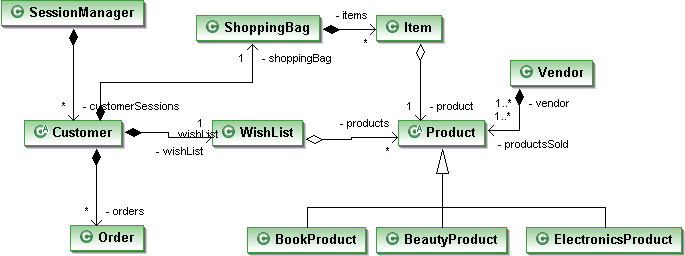
\includegraphics[width=\textwidth]{images/myonlineshop.png}%
\caption{A simple online shop application}%
\label{fig:shop}%
\end{figure}

Below, we outline the architecture and design of an online store application. We use this scenario to give examples of categorizing objects according to how they are used and how to use these categories in the implementation of concerns. It must be noted that we intend to support the addition of \emph{unanticipated} concerns, i.e., the program code is not prepared to support abstractions, like specific object categories, required by the new concerns.
At the end of this section, we conclude requirements for solving the encountered challenges in these examples.

\paragraph{Example Architecture}
An online shop is a sophisticated web application and objects of the same type can exist at different stages of the life-cycle. In Figure \ref{fig:shop} the static structure of a simplified online shop is shown. When a new user logs in, \texttt{SessionManager} creates a \texttt{Customer} object to represent the user's session. A customer has a \texttt{ShoppingBag} and a \texttt{WishList}. The abstract class \texttt{Product} is super-type of all products in the shop and represents product data. The \texttt{Product}'s subclasses are \texttt{BeautyProduct}, \texttt{BookProduct} etc. When the customer selects a product and clicks ``add to shopping bag'', a new \texttt{Item} instance is created and added to the \texttt{ShoppingBag} object; the \texttt{Item} instance contains the \texttt{Product} and how many of that \texttt{Product} are added. A customer can add/remove items from his shopping bag. When the shopping is finished the \texttt{checkOut()} method is invoked on \texttt{Customer}, which returns an object of type \texttt{Order}. To complete the order the customer has to provide some information and finalize the order. A \texttt{Customer} can also \texttt{Product}s to his \texttt{WishList}; the \texttt{WishList} holds a list of \texttt{Products}, whereas \texttt{ShoppingBag} holds a list of \texttt{Item}s.

\paragraph{Unanticipated Extensions}
Let's assume a new requirement for applying a happy-hour discount is introduced. The discount should be applied at check-out to \texttt{Item}s which have been added to a customer's shopping bag between certain hours.
In order to realize this extension in an OO-approach, one needs to invasively change the system code: First we need to keep a set of items that were added to a shopping bag within the timing condition. Then when the user finally checks out, we have to apply the discount to the items in the set. Listing \ref{lst:happyhour} shows that we need to insert code in multiple places to satisfy the new requirement. First a set, called \texttt{happyItems}, is created (Line 1), to keep track of items that are added during the happy-hour. In the \texttt{addToShoppingBag} method the timing condition is checked, and when the condition is satisfied the created \texttt{Item} is added to \texttt{happyItems} (Lines 6--7).  Finally in the \texttt{checkOut} method the discounts are applied to the items in \texttt{happyItems} (Line 18). 

\begin{lstlisting}[float, caption={A Java implementation of Happy-hour discount rule}, label={lst:happyhour}]
Set<Item> happyItems = createSet();
public boolean addToShoppingBag(Product p, int amount)
{
	Item item = ItemFactory.createItem(p,amount);
	
	if('timing condition')
		items.put(item)
	
	this.shoppingBag.add(item);
}
public boolean removeFromShoppingBag(Item item, int amount)
{
	...
	items.remove(item);
}
public checkOut()
{
	ProductManager.applyHappyHourDiscount(items, happyItems);
}
\end{lstlisting}

Even for a single discount rule, the code for the discount concern and the book-keeping that comes with it creates cluttering. If we would like to apply multiple discount rules for the \emph{check out} event, this implementing style is clearly not suitable.
An aspect-oriented implementation can offer a better solution by encapsulating the concern in an aspect. In Listing \ref{lst:happyhouraop} the \texttt{newItem} pointcut (Lines 2--4) selects join-points where a customer adds a product to his bag: a new \texttt{Item} is created in the \texttt{addToShoppingBag} method. The advice is executed when \texttt{newItem} is matched; after returning the new \texttt{Item}, the timing condition is checked and if it holds it is added to \texttt{happyItems}. \textbf{the condition should better be checked in an if-pointcut.}
We also define the \texttt{removeItem} pointcut (Lines 5--7) and advise it (Lines 15--18) to remove an item from \texttt{happyItems} if it is removed from a shopping bag.
Finally, we define a pointcut for selecting the \texttt{Customer.checkOut()} join-point (Line 8) and before the method is executed we apply the discount to items in \texttt{happyItems}.
An AO implementation, although offers a non-invasive solution, also suffers from boilerplate code written for book-keeping. 

\begin{lstlisting}[float, caption={An Aspectj implementation of Happy-hour discount rule}, label={lst:happyhouraop}]
Set<Item> happyItems = createSet();
pointcut newItem(Item item): 
		call(* ItemFactory.createItem(..)) && 
		withincode(* Customer.addToShoppingBag(..));
pointcut removeItem(Item item): 
	call(* Customer.removeFromShoppingBag(..)) && 
	args(item);
pointcut checkOut(Customer customer): call(* Customer.checkOut()) &&
        target(customer);

after() returning(Item item): newItem(item)
{
	if('timing condition')
		happyItems.put(item);
}
after(Item item): removeItem(item)
{
	happyItems.remove(item);
}
before():checkOut(Customer customer)
{
	ProductManager.applyHappyHourDiscount(customer.items, happyItems);
}
\end{lstlisting}

\paragraph{Discussion and Requirements}

AOP already helps to localize the concern, e.g., of a specific discount policy, and to add it without the need to modify existing code.
But most of the implementation of the discount policy as shown in Listing \ref{lst:happyhouraop} consists of boilerplate code. Only the definition of the pointcut and the advice to \texttt{checkOut} are concern-specific.
Furthermore reusing existing sets by specifying subsets or composing them is not conveniently supported at all; e.g., if we want to find the subset of \texttt{BeautyProduct}s in a set of \texttt{Product} objects, we have to iterate over it and check instance types to create a new set.

In order to overcome the shortcomings of existing approaches, we need a way to declaratively select objects based their life-cycle phases, where the beginning and the end of a phase is marked by events. From the scenario described above and from our experience, we conclude the following requirements:

\begin{enumerate}[{Requirement}1{:}]
\item A declarative way of reifying a set of objects by defining add/remove conditions must be provided.
\item Since objects may recursively enter a life-cycle phase, it must be counted how often the begin and end events have occurred for each object.
\item Add/Remove expressions must select events and specify which object form the context of the event is selected.
\item It must be possible to access the set of objects which currently comprises an object category and to be notified when the set changes.
\item A declarative way to refine existing sets to subsets, supersets or compositions is required.
\item Validity should be ensured for subset and superset refinement, and composition in general, either by construction or through compile-time checks.
\end{enumerate}


\section{Instance Pointcuts}
\label{sect:ip}
Instance pointcut is a declarative language construct that is used to reify and maintain a set of objects of a specified type, with the ability to select them over a period marked by events in their life-cycle, modularizing the object selection concern and making it declarative. 
%The purpose of instance pointcuts is to  let the user to make focused selections, therefore offering a different level of modularity. 
 
In the remainder of this section, we will explain instance pointcuts in detail. We have implemented a prototype by extending AspectJ. Throughout the section code examples of instance pointcuts will contain AspectJ pointcut expression.

%\todo[inline]{maybe section outline summarizing main features}
%\missingfigure{Static Structure of instance pointcuts}

\subsection{Instance Pointcut Language Features}
\label{sec:features}

A concrete instance pointcut definition consists of a left hand-side and a right-hand side (Figure~\ref{fig:grammar1}, rule 1). 
On the left-hand side the pointcut's name and a type reference of interest is declared. 
An instance pointcut does not declare pointcut parameters; it has a single implicit parameter called \lstinline{instance} of the declared type. 
On the right-hand side a pointcut expression selects the desired events from join points and then binds the exposed object (represented by \lstinline{instance} parameter) as a member of the instance pointcut's set. 
An instance pointcut is a \emph{static aspect member}. % (Listing~\ref{lst:member}).% and they can only be declared in a singleton aspect.

\begin{figure}[h!]
\begin{grammar}
<instance pointcut> ::= `instance pointcut' <name> `<' <instance-type> `>' `:'
<ip-expr> (`UNTIL' <ip-expr>)? 

<ip-expr> ::= <after-event> `||' <before-event> \alt <before-event> `||' <after-event> \alt <after-event> \alt <before-event>

<after-event> ::= `after' `('<pointcut-expression>`)'

<before-event> ::= `before' `('<pointcut-expression>`)'
\end{grammar}
\caption{Grammar definition for instance pointcuts}
\label{fig:grammar1}
\end{figure}

%\begin{lstlisting}[float=h!, caption={An instance pointcut declaration in an aspect}, label={lst:member}]
%aspect MyAspect{
	%static instance pointcut products<Product> ...
%}
%\end{lstlisting}
%It is also possible to declare an abstract instance pointcut, by leaving out the right hand side and placing the \emph{abstract} modifier at the beginning of the declaration and not defining a pointcut expression. Abstract instance pointcuts are used when execution details are not yet clear but the instance set to be created and its instance type are determined.

\subsubsection{Add/Remove Expressions}
\label{sect:addrem}
Instance pointcuts implicitly perform add to set and remove from set operations, when certain events are matched. An instance pointcut expression, which consists of two sub-expressions that are separated by the \lstinline{UNTIL} keyword,  defines the events and matching conditions (Figure~\ref{fig:grammar1}, rule 1). One of the sub-expressions is the \emph{add expression} that selects events which expose the instances to be added to the instance pointcut set; an event selected by the add expression marks the beginning of the life-cycle phase of interest. After the \lstinline{UNTIL} clause an optional sub-expression called the \emph{remove expression} can be defined,  which specifies when to remove which object: it selects the event that marks the end of the life-cycle phase of interest. When the remove expression is not defined, then the object is kept in the set until it \emph{dies}.

 
In AspectJ join points mark \emph{sites} of execution; a join point by itself does not define an event. 
Pointcut expressions select join points and pointcuts are used with advice specifications to select a particular event in that join point. The shortcomings of this region-in-time model is discussed by Masuhara et al.\ in \cite{masuharafine}.
We combine pointcut expressions with advice specifiers and obtain \emph{expression elements}. Each expression element contains a pointcut expression, which matches a set of join points. Then, from these join points, according to the advice specifier the before or after events are selected.
Both add and remove expressions are composed of expression elements. The expression elements can be one of two types, \emph{before element} and an \emph{after element} (Figure~\ref{fig:grammar1}, rule 3-4). A sub-expression (add/remove expression) contains at least one \emph{expression element} and at most two. In Figure~\ref{fig:grammar1} the second grammar rule depicts this statement. 

In Figure~\ref{fig:grammar1} rules 3 and 4 contains the $\langle pointcut-expression\rangle$ rule which represents an AspectJ pointcut expression. However we have introduced a restriction that in every pointcut expression there must be a binding predicate (args, target etc.) that bind the \lstinline{instance} parameter and the binding predicates are extended to include the \lstinline{returning} clause. The \lstinline{returning} clause binds the returned variable by a method or a constructor. AspectJ only allows it to be used with an after advice, specifically known as \texttt{after returning}. 

In an instance pointcut expression, it is only possible to \emph{OR} a before event with an after event. 
The \emph{before} clause selects the start of executing an operation (i.e., the start of a join point in AspectJ terminology) and the \emph{after} clause selects the end of such an execution. 
For two operations that are executed sequentially, the end of the first and the start of the second operation are treated as two different events. Thus, the before and after clauses select from two disjoint groups of events and the conjunction of a before and an after clause will always be empty.

\begin{lstlisting}[float=h!, caption={A basic instance pointcut declaration with add and remove expressions}, label={lst:basic}]
static instance pointcut surpriseDiscount<Product>: 
	after(call(* ProductManager.submitDiscount(..)) 
	&& args(instance, SurpriseDiscount)) 
	UNTIL 
	after(call(* ProductManager.withdrawDiscount(..)) 
	&& args(instance, SurpriseDiscount));
\end{lstlisting}

The instance pointcut in Listing~\ref{lst:basic} shows a basic example. The left-hand side of the instance pointcut indicates that the pointcut is called \lstinline{surpriseDiscount} and it is interested in selecting \lstinline{Product} objects. 
On the right hand side, there are two expressions separated by the \lstinline{UNTIL} keyword. The first one is the add expression. It selects join-point marked by the method \textsf{submitDiscount} and from the context of this event it exposes the \lstinline{Product} object with the \lstinline{args} clause and binds it to the \lstinline{instance} parameter. 
The second one is the remove expression and it selects the after event \textsf{withdrawDiscount} call and exposes the \lstinline{Product} instance in the method arguments and binds it to the \lstinline{instance}.
This pointcut is the solution of the set maintenance problem presented in the motivation (section~\ref{sect:motivation}).
 
As well as the regular AspectJ binding predicates (\textsf{\textbf{args, this, target}}) we also support the usage of \texttt{\textbf{returning}} to bind the returned value of a method. 
If the \lstinline{instance} parameter is bound by the \lstinline{returning} clause then it has to be in an after event, since the returned value is only available after a method finishes execution. 

\emph{Note that instance pointcuts do not keep objects alive}, as instance pointcuts are non-invasive constructs, which do not affect the program execution in any way. So even if the remove expression was not defined for the \lstinline{customers} instance pointcut, when the \lstinline{Customer} instances are collected by the garbage collector, they are removed from the set. 

\subsubsection{Multisets}
An instance pointcut reifies an object set as a \emph{multiset}. Multisets allow multiple appearances of an object. The formal definition of a multiset is as follows:

\begin{mydef}
\label{def:multiset}
A multiset is a pair $(X, f)$, where $X$ is a set and $f$ is a function mapping $X$ to the cardinal numbers greater than zero. $X$ is called the underlying set of the multiset, and for any $x \in X$, $f(x)$ is the multiplicity of $x$.

Note that we do not allow a multiplicity of zero or infinite.
\end{mydef}

The instance pointcut shown in Listing~\ref{lst:discounted} selects \lstinline{Product} instances, which are applied a \texttt{Discount}. The remove expression removes a \lstinline{Product} instance if the \texttt{Discount} is removed from that \texttt{Product}. With this pointcut we would like to represent the currently discounted products. Multiset makes sure that \lstinline{Product}s can be added for each discount submission operation. When the same product is added with different types of discounts, and if one of discounts are removed, then still one entry of that instance is left in the set.  If instance pointcuts only supported a set then as soon as a discount is removed from a product, its only copy would be removed and it would appear as if there are no more discounts on that product. 

\begin{lstlisting}[float=h!, caption={An instance pointcut utilizing multiset property}, label={lst:discounted}]
static instance pointcut multi_discount<Product>: 
	after(call(* ProductManager.submitDiscount(..)) 
	&& args(instance)) 
	UNTIL 
	after(call(* ProductManager.withdrawDiscount(..)) 
	&& args(instance));
\end{lstlisting}


\subsection{Refinement and Composition}

Instance pointcuts can be referenced by other instance pointcuts, they can be refined in terms of instance type and composed together to create new instance pointcuts. 

\subsubsection{Referencing and Type Refinement}
Instance pointcuts are referenced by their names. Optionally the reference can also take an additional statement for \emph{type refinement}, which selects a subset of the instance pointcut of refined type. Type refinements require that the refined type is a subtype of the original instance type. For example the instance pointcut \lstinline{surpriseDiscount} (Listing~\ref{lst:basic}) can be refined as in the following:
\begin{lstlisting}[float=h!]
static instance pointcut surpriseDiscountBeauty<BeautyProduct>: 
	surpriseDiscount<BeautyProduct>
\end{lstlisting}

This selects the subset of \lstinline{BeautyProduct} instances from the set of \lstinline{Product} instances selected by the \lstinline{surpriseDiscount} instance pointcut. 
Note that this notation will also select subtypes of \lstinline{BeautyProduct}. 

\subsubsection{Instance Pointcut Expression Extension}
In subsection~\ref{sect:addrem} we have introduced the instance pointcut expression, which consists of a two sub-expressions (add and remove expression). The expression elements forming these sub-expressions can be accessed individually to be extended by concatenating other primitive pointcuts. 

\subsubsection{Instance Pointcut Composition}

Instance pointcuts reify sets, for this reason the composition of instance pointcuts are defined in terms of set operations: \emph{intersection and union}. 
In Figure~\ref{fig:grammar2}, an extended version of the grammar definition is shown. 
A new instance pointcut can be defined by declaring an instance pointcut reference and a partial set composition expression.  In order to declare a set intersection the keyword \texttt{inter} and to declare a set union the keyword \texttt{union} is used. Throughout the text we will use the mathematical symbols for these operations, $\cap$ as intersection and $\cup$ as union.

\begin{figure}[h]
\begin{grammar}
<instance-pointcut> ::= `instance pointcut' <name> `<' <instance-type> `>' `:'
... \alt <ip-ref> <partial-set-composition>*

<partial-set-composition> ::= <set-operator> <ip-ref>

<set-operator> ::= `inter' \alt `union'

<ip-ref> ::= <name> \alt <name>(`<' <refined-instance-type> `>')?

%\ldots
\end{grammar}
\caption{Syntax for instance pointcut composition}
\label{fig:grammar2}
\end{figure}

The type of an instance pointcut must correspond to the type of the composed instance pointcuts. For a composition of two instance pointcuts, the type of the composed one can be determined depending on the relation of the types of the component instance pointcuts and the type of composition. Consider the representative type hierarchy in Figure~\ref{fig:types}: \lstinline{R} is the root of the hierarchy with the direct children \lstinline{A} and \lstinline{B} (i.e., these types are siblings); \lstinline{C} is a child of \lstinline{B}. Table~\ref{table1} shows four distinct cases: Either the type of one of the instance pointcuts is a super type of the other one's type (second row), or both types are unrelated (third row); and the composition can either be $\cap$ (third column) or $\cup$ (fourth column).

When composing two instance pointcuts with types from the same hierarchy, the type of the composition is the more specific type (\lstinline{C} in the example) for an $\cap$ composition and the more general type (\lstinline{B}) for an $\cup$ composition.
When composing two instance pointcuts with sibling types, for the $\cap$ operation the resulting composition cannot select any types since the types \lstinline{A} and \lstinline{B} cannot have a common instance. The $\cup$ operation will again select a mix of instances of type \lstinline{A} and \lstinline{B}, thus composed instance pointcut must have the common super type, \lstinline{R} in the example.


%The composition also has an effect on the types of the instances that are added to the set. To better explain this effect we have created a small example, where a members of a simple type hierarchy (Figure~\ref{fig:types}) are used in instance pointcuts. Table~\ref{table1} shows four distinct cases. In the first case we compose two instance pointcuts \lstinline{pc1<B>} and \lstinline{pc2<C>} with an \&\& operation, the resulting instance pointcut from this composition can only select the narrower type \lstinline{C} since the composed expression is stricter and the type restriction comes from \lstinline{pc2}. However with $\|$ operation we can capture \lstinline{B} types as well as \lstinline{C} types, so the resulting composition will select a mixture. In the second row a case with sibling types are shown. For the \&\& operation the resulting composition cannot select any types since the types \lstinline{A} and \lstinline{B} cannot have a common instance. The $\|$ operation will again select a mix of instances of type \lstinline{A} and \lstinline{B}, then the instance type for the composed instance pointcut should be \lstinline{R} to contain the subtypes.

\begin{figure*}%[h]
\centering
\subfloat[A simple type hierarchy]{
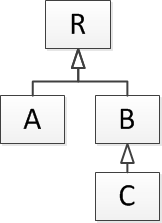
\includegraphics[width=0.10\textwidth]{images/types.png}
\label{fig:types}
}
\hspace{40pt}
\subfloat[Instance pointcut compositions and effect on the captured instance type]{ 
\label{table1}
\centering
\begin{tabular}[b]{|p{1cm}|p{1cm}|p{1cm}|p{1cm}|}
\hline 
pc1 type & pc2 type     &$\cap$         &$\cup$  \\[1ex]
\hline
B & C & C & B \\[1ex]
\hline
B & A & $\emptyset$ & R\\[1ex]
\hline 
\end{tabular}
}
\vspace{10pt}
\caption{An example to illustrate composition's effect on types}
\label{fig:compotypes}
\end{figure*}


\paragraph{Semantics}
The composition of two instance pointcuts is computed by composing the content of their sets \emph{at the time of the composition}. The result is an instance pointcut which monitors the composing instance pointcuts and updates the composition sets accordingly. We have defined two composition operators for instance pointcuts, union and intersection. Since instance pointcuts are reified as multi-sets, these operations are different from the regular set operations.

\begin{mydef}
\label{def:inun}
Assume $(X, f)$ and $(Y, g)$ are multisets. 

The \textbf{intersection} of these sets is defined as $(V, h)$ where, 
\[V = X \cap Y\] and
$\forall v \in V$ the multiplicity of $v$ is defined as \[h(v) =  min(f(x),g(x))\]

The \textbf{union} of these sets is defined as $(Z, i)$ where, 
\[Z = X \cup Y\] and
$\forall z \in Z$ the multiplicity of $z$ is defined as \[i(z) =  max(f(x),g(x))\]
\end{mydef}

The objects in an instance pointcut's set can be added and removed at certain events, which makes the contents of the set dynamic. Therefore the composition operation requires monitoring of the component sets.  Figure~\ref{fig:interunionvis} presents a visualization of these operations. The small triangles represent the adding of an object to the instance pointcut set and the small circles represent the removal. The ellipses represent the instance pointcut set, and their major axes sit between the add and remove events of the corresponding instance pointcut (Ipc1 and Ipc2). The line represents execution flow of a \emph{single} object. This object is first added to the set of Ipc1 at the first dark triangle. Between this event and Ipc2's add event (light triangle):
\[Ipc1 \cup  Ipc2 = Ipc1\]
\[Ipc1 \cap Ipc2 = \emptyset\]

When the object is added to Ipc2's set at the light triangle then their intersection is no longer empty and the union no longer consists of only Ipc1's elements. The result of the union and the intersection is computed according to definition~\ref{def:inun}. When the object is removed from Ipc1's set (small dark circle) then the intersection is once again empty. Of course this abstract example only shows a simple case where an instance pointcut selects only one join-point for selecting and one joinpoint for removing an instance. In practice instance pointcuts can be more complex, where they can match multiple events which alters their sets. 

\begin{figure}
	\centering
		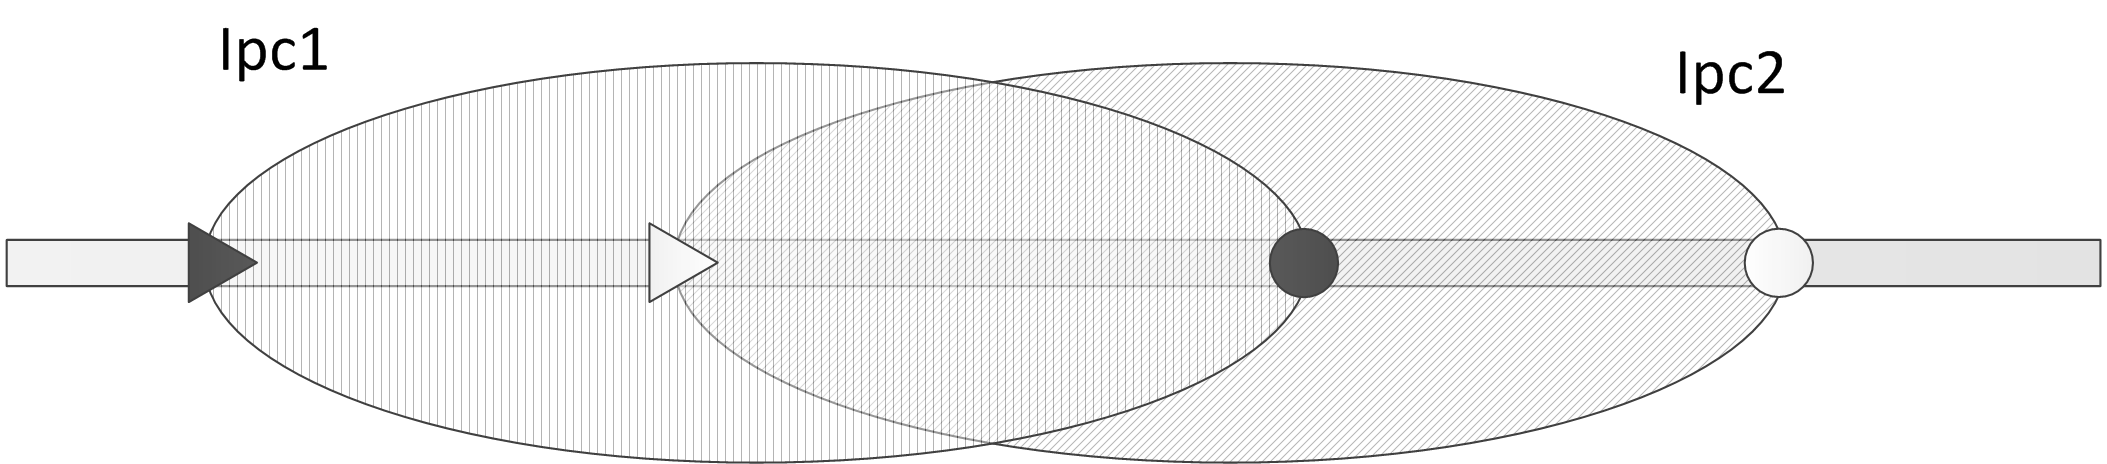
\includegraphics[width=\columnwidth]{images/interunionvis.png}
	\caption{Intersection and Union of two instance pointcuts}
	\label{fig:interunionvis}
\end{figure}




%An instance pointcut can have at most four expression elements; before add ($ba$) and after add ($aa$) form the add expression and, before remove ($br$) and after remove($ar$) form the remove expression. Let us define an instance pointcut as $IP = ba_{IP}\;\|\;aa_{IP}\;\textrm{UNTIL}\;br_{IP}\;\|\;ar_{IP}$. Each element contains a pointcut expression referred with the notation $ba_{IP}\_expression$. 
%
%\begin{align}
	%IP1 = ba_{IP1}\;\|\;aa_{IP1}\;%\textrm{UNTIL}\;br_{IP1}\;\| ar_{IP1} 
%\label{i1}	\\
	%IP2 = ba_{IP2}\;\|\;aa_{IP2}\;%\textrm{UNTIL}\;br_{IP2}\;\| ar_{IP2}
%\label{i2}
%\end{align}
%
%Let us define a new instance pointcut as; $IP3 = IP1\;\textrm{\&\&}\;IP2$. By distributivity this operation results in the following formulation:
%
%\begin{align}
%\begin{split}
%IP3 \rightarrow \textrm{add expression} =& \left( ba_{IP1}\;\textrm{\&\&}\;ba_{IP2}\right)\;\\ 
							%&\|\;\left( ba_{IP1}\;\textrm{\&\&}\;aa_{IP2} \right)\;\\
%&\|\;\left( aa_{IP1}\;\textrm{\&\&}\;aa_{IP2} \right)\;\\
%&\|\;\left( aa_{IP1}\;\textrm{\&\&}\;ba_{IP2} \right) 
%\label{i3add}
%\end{split}
%\end{align}
%
%The composition of before and after event via \&\& will be empty as explained at the beginning of this section. Composing two events of the same type with a logical operator is formulated as follows, where event is either \emph{before} or \emph{after}:
%\begin{align*}
%event(exp_1)\;\&\&\;event(exp_2) = event(exp_1\;\&\&\;exp_2) \\
%event(exp_1)\;\|\;event(exp_2) = event(exp_1\;\|\;exp_2)
%\end{align*}
%
%Note that we do not analyze expressions to verify their composition and leave that to the AspectJ compiler. For example AspectJ does not allow use of different binding predicates in the composed expression and this is also a limitation of instance pointcut composition. 
%
%Finally IP3 becomes:
%\begin{align}
%\begin{split}
%IP3 =& \overbrace{\left( ba_{IP1}\;\textrm{\&\&}\;ba_{IP2}\right)}^{ba_{IP3}}\;\|\;\overbrace{\left( aa_{IP1}\;\textrm{\&\&}\;aa_{IP2} \right)}^{aa_{IP3}}\;\\
%\label{ip3step}
%\end{split}
%\end{align}
%
%If IP1 and IP2 define remove expressions, then the composed instance pointcut IP3 will become:
%
%\begin{align}
%\begin{split}
%IP3 =& \overbrace{\left( ba_{IP1}\;\textrm{\&\&}\;ba_{IP2}\right)}^{ba_{IP3}}\;\|\;\overbrace{\left( aa_{IP1}\;\textrm{\&\&}\;aa_{IP2} \right)}^{aa_{IP3}}\;\\
%&\textrm{UNTIL} \\
%&\underbrace{\left( br_{IP1}\;\|\;br_{IP2}\right)}_{br_{IP3}}\;\|\;\underbrace{\left( ar_{IP1}\;\|\;ar_{IP2} \right)}_{ar_{IP3}}\;\\  
%\label{ip3step}
%\end{split}
%\end{align}
%
%Notice that the remove expressions are applied $\|$ instead of \&\&. If we narrow down the removal criteria by \&\& then it is possible that some objects which are added will not be removed. By keeping the removal criteria for both of the composed instance pointcuts, we ensure that all the added objects can be removed. So we can say that the \&\& and the $\|$ operations only effect the expression elements in the add expression.
%
%
%If we define another instance pointcut as $ IP4 = IP1\;\|\;IP2$, after performing the above formulations we get:
%\begin{align}
%\begin{split}
%IP4 =& \overbrace{\left( ba_{IP1}\;\|\;ba_{IP2}\right)}^{ba_{IP4}}\;\|\;\overbrace{\left( aa_{IP1}\;\|\;aa_{IP2} \right)}^{aa_{IP4}}\;\\
%&\textrm{UNTIL} \\
%&\underbrace{\left( br_{IP1}\;\|\;br_{IP2}\right)}_{br_{IP4}}\;\|\;\underbrace{\left( ar_{IP1}\;\|\;ar_{IP2} \right)}_{ar_{IP4}}\;\\  
%\label{ip3step}
%\end{split}
%\end{align}
%
%\begin{align}
%\begin{split}
%IP3 \rightarrow \textrm{remove expression}  =& \left( br_{IP1}\;\|\;br_{IP2}\right)\; \\
%&\|\;\left( br_{IP1}\;\|\;ar_{IP2} \right)\;\\
%&\|\;\left( ar_{IP1}\;\|\;ar_{IP2} \right)\;\\
%&\|\;\left( ar_{IP1}\;\|\;br_{IP2} \right) 
%\label{i3remove}
%\end{split}
%\end{align}
%
%Using the same composition principles, instance pointcuts can also be composed with expression elements, to refine or broaden the instance pointcut scope. For the instance pointcut IP5 which is defined as:
%
%\begin{align}
%\begin{split}
%IP5 & = IP1\;||\;(ba_{new}\;UNTIL\;ar_{new}) \\
   %& = \overbrace{\left( ba_{IP1}\;\|\;ba_{new}\right)}^{ba_{IP5}}\;\|\;\overbrace{\left( aa_{IP1} \right)}^{aa_{IP5}}\;\\
%&\textrm{UNTIL} \\
%&\underbrace{\left( br_{IP1}\right)}_{br_{IP5}}\;\|\;\underbrace{\left( ar_{IP1}\;\|\;ar_{new} \right)}_{ar_{IP5}}\;\\  
%\end{split}
%\end{align}
%
%Let us illustrate these concepts with a concrete example. The first instance pointcut  (\lstinline{lowSelling})  shown in Listing~\ref{lst:refmain} selects the \lstinline{Product}s which are marked as \emph{low-selling} by the \lstinline{OnlineShop} class and remove those products which are discontinued by the \lstinline{Vendor}. The second instance pointcut (\lstinline{wishList})  selects the \lstinline{BookProduct}s which are added to the wishlist of a \lstinline{Customer} and removes them when they are out of the wishlist.
%
%\begin{lstlisting}[float=h!, caption={Two instance pointcuts composed to obtain a new one}, label={lst:refmain}]
%static instance pointcut lowSelling<Product>: 
	%after(call(* OnlineShop.setLowSelling(..)) &&
				%args(instance)) 
	%UNTIL 
	%before(call(* Vendor.discontinue(..)) &&
				%args(instance));
				%
%static instance pointcut wishList<BookProduct>: 
	%after(call(* Customer.addToWishList(..)) &&
				%args(instance)) 
	%UNTIL 
	%before(call(* Customer.removeFromWishList(..)) &&
				%args(instance)) ;
				%
%static instance pointcut composition<Product>: 
	%lowSelling || purchase;
%\end{lstlisting}
%
%The new instance pointcut \lstinline{composition} is the result of an $\|$ operation between \lstinline{lowSelling} and \lstinline{wishList}. Then the add and remove expressions of \lstinline{composition} is created by factoring out the \lstinline{args} pointcut and the composed instance pointcut expression is shown in Listing~\ref{lst:newpc}. 
%
%\begin{lstlisting}[float=h!, caption={The new instance pointcut after composition}, label={lst:newpc}]
%static instance pointcut composition<Product>: 
	%after((call(* OnlineShop.setLowSelling(..)) || call(* Customer.addToWishList(..))) && 
				%args(instance)) 
	%UNTIL 
	%before((call(* Vendor.discontinue(..)) || call(* Customer.removeFromWishList(..))) && 
				%args(instance))
%\end{lstlisting}
%
%
%Similarly we can define a new instance pointcut (Listing~\ref{lst:comp2}), this time by composing an instance pointcut with an expression element, then the \lstinline{composition2} instance pointcut has the pointcut expression shown in Listing~\ref{lst:comp2exp}.
%
%\begin{lstlisting}[float=h!, caption={An instance pointcut and an expression is composed}, label={lst:comp2}]
%static instance pointcut composition2<Product>: 
	%lowSelling && 
	%after(if(instance.getPrice() > 10)) 
	%UNTIL 
	%before(call(* OnlineShop.removeFromShop(..)) && 
				%args(instance));
%\end{lstlisting}
%
%
%\begin{lstlisting}[float=h!, caption={The composition2 instance pointcut after composition}, label={lst:comp2exp}]
%static instance pointcut composition2<Product>: 
	%after(call(* OnlineShop.setLowSelling(..)) && 
				%args(instance) && 
				%if(instance.getPrice() > 10)) 
	%UNTIL
	%before((call(* Vendor.discontinue(..)) || 
				%call(* OnlineShop.removeFromShop(..))) && 
				%args(instance));
%\end{lstlisting}

\subsubsection{Checking}
Instance pointcuts also have checking mechanisms to warn the user for potential errors and enforcing some constraints. In some cases it can be possible to identify if a set is empty or not during compile time, for example when the pointcut expressions defined in expression elements of the instance pointcut do not match any join points. 
%For the subset and superset relationships, type checking is performed to see if they satisfy the typing restrictions. 
Currently more advanced checks and verifications are still future work.

\subsection{Using Instance Pointcuts}
Up to now we have explained the syntax and semantics for instance pointcuts. In this section we will explain how to use instance pointcut in the context of an AO languge, namely, AspectJ. The instance pointcut defined in Listing~\ref{lst:usage} maintains a set of \lstinline{Product}s that are currently out of stock.

\begin{lstlisting}[float=h!, caption={An instance pointcut for out of stock products}, label={lst:usage}]
aspect MyAspect{
	static instance pointcut outOfStock<Product>: 
		after(call(* Product.outOfStock(..)) && 
					target(instance)) 
		UNTIL 
		after(call(* Vendor.stock(..)) 
					&& args(instance));
	...
}
\end{lstlisting}

\subsubsection{Set Access}
Instance pointcuts reify a set and this set can be accessed through a static method, which has the same name as the instance pointcut identifier. Then the \emph{read} methods of the collection interface can be used to retrieve objects from the set. Write methods are not allowed since it creates data inconsistencies and it may result in concurrent modification exceptions. 

%The set can also be referenced with a type refinement, which will return a subset of the original set with objects of refined type. 

\begin{lstlisting}[float=h!, caption={Calculate a damage estimate for out of stock products}, label={lst:setaccess}]
public static double calculateDamages()
{
	double damage = 0;
	for(Product p: MyAspect.outOfStock())~\label{lst:setaccess:access}~
		damage = damage + p.getPrice();
	return damage;
}
\end{lstlisting}

In Listing~\ref{lst:setaccess},  a method called \lstinline{calculateDamages} is defined in \lstinline{MyAspect}. This method calculates a rough estimate of the shop's damages when products are out of stock. On line~\ref{lst:setaccess:access}, the for loop iterates over the \lstinline{outOfStock}'s set, which is accessed as a static method.


\subsubsection{Set Monitoring}
An instance pointcut definition defines two set change events, an add event and a remove event. In order to select the join points of these events, every instance pointcut definition automatically has two implicit regular pointcuts. These implicit pointcuts have the following naming conventions, $\langle name \rangle\_add, \langle name \rangle\_remove$, where $\langle name \rangle$ is the name of the instance pointcut. These pointcuts allow the user to access the set change event and the object to be added or removed. In Listing~\ref{lst:monitor1}, a before advice using the \lstinline{outOfStock_add} pointcut is shown. When a product is marked out of stock then it is added to the set, this advice uses the \lstinline{Product} instance to be added and notifies the related \lstinline{Vendor} that the product is out of stock.

\begin{lstlisting}[float=h!, caption={Set monitoring pointcut used to notify vendors}, label={lst:monitor1}]
before(Product p): outOfStock_add(p)
{
	OnlineShop.notifyVendor(p.getVendor, STOCK_MSG);
}
\end{lstlisting}

\subsection{Compilation of Instance Pointcuts}

%TODO: access method IPAspect.ipc vs. IPAspect.ipc()

We have implemented the instance pointcut language with the EMFText language workbench.
For this purpose, we have defined the AspectJ grammar by using JaMoPP\footnote{JaMoPP: Java Model Parser and Printer, see \url{http://jamopp.inf.tu-dresden.de}}~\cite{jamopp2010} as the foundation and extended it with the grammar for instance pointcuts which was presented interspersed with the rest of this section.
During compilation, the instance pointcut definitions are transformed into semantically equivalent source code, the remaining definitions are preserved as they are; the result is compiled with the AspectJ compiler.
A goal for our compiler implementation is to support modular compilation.
This means to compile an aspect with instance pointcuts that refer to instance pointcuts defined in other aspects, it must be sufficient to know their declaration (i.e., the name and type); it should not be necessary for the compiler to know the actual expression or the referenced instance pointcuts.

The Listing~\ref{lst:management} shows the code which is generated by our compiler for managing the data of an instance pointcut; the variables \emph{\$\{Type\}} and \emph{\$\{ipc\}} stand for the instance pointcut's type and name, respectively.
First, a \lstinline{WeakHashMap} is defined for storing the instances currently selected by an instance pointcut (cf.\ line~\ref{lst:management:map}).
We use weak references to avoid keeping objects alive which are not reachable from the base application anymore.
The keys of the map are the objects which are selected by the instance pointcut; the mapped value is a counter of how often the object has been selected by the instance pointcut.
The generated method \emph{\$\{ipc\}} returns all objects which are currently mapped (cf.\ lines~\ref{lst:management:data:start}--\ref{lst:management:data:end}).

Furthermore, methods are generated to increase or decrease the counter of selected objects; if an object does not have an associated counter yet or the counter reached zero, the object is added to or removed from the map, respectively (cf.\ lines~\ref{lst:management:bookkeeping:start}--\ref{lst:management:bookkeeping:end}).
After having performed their operations, both methods invoke an empty method, passing the added or removed object.
We generate a public, named pointcut selecting these calls, exposing the respective events (cf.\ lines~\ref{lst:management:added:pc} and~\ref{lst:management:removed:pc}).

\lstset{
morecomment=[s][\itshape]{\$\{}{\}},
moredelim=[is][\rmfamily\itshape]{|}{|},
deleteemph={instance},
escapechar={~}
}
\begin{lstlisting}[float, caption={Template of generated code for instance set management.},label=lst:management]
private static WeakHashMap<${Type}, Integer> ${ipc}_data = new WeakHashMap<${Type}, Integer>(); ~\label{lst:management:map}~

public static Set<${Type}> ${ipc}() { ~\label{lst:management:data:start}~
	return Collections.unmodifiableSet(${ipc}_data.keySet());
} ~\label{lst:management:data:end}~

public static void ${ipc}_addInstance(${Type} instance) { ~\label{lst:management:bookkeeping:start}~
	|increase counter associated with instance by the ${ipc}_data map|
	${ipc}_instanceAdded(instance); ~\label{lst:management:added}~
}

public static void ${ipc}_removeInstance(${Type} instance) {
	|decrease counter associated with instance by the ${ipc}_data map|
	|if the counter reaches 0, remove instance from the map|
	${ipc}_instanceRemoved(instance); ~\label{lst:management:removed}~
} ~\label{lst:management:bookkeeping:end}~

private static void ${ipc}_instanceAdded(${Type} instance) {}

private static void ${ipc}_instanceRemoved(${Type} instance) {}

public pointcut ${ipc}_add(${Type} instance) : call(private static void Aspect.${ipc}_instanceAdded(${Type})) && args(instance); ~\label{lst:management:added:pc}~
public pointcut ${ipc}_remove(${Type} instance) : call(private static void Aspect.${ipc}_instanceRemoved(${Type})) && args(instance); ~\label{lst:management:removed:pc}~
\end{lstlisting}

Next, these bookkeeping methods have to be executed at the events specified in the instance pointcut expression.
At first sight, realizing this by generating AspectJ pointcuts and advice seems to be a reasonable solution.
However, the way AspectJ handles binding values and restricting their types in pointcuts prevents a modular compilation of instance pointcuts.

An instance pointcut expression can be transformed into several named AspectJ pointcuts which bind a single value, the \emph{instance}.
However, in AspectJ the result value of a join point is bound by the \lstinline{after returning} keyword in the advice definition instead of the pointcut definition.
Therefore, the generated AspectJ code depends on which value is bound; this means when another pointcut is referenced then the binding predicate of the referenced pointcut should be known.
Also it is not possible to work around this, using AspectJ's reflective \lstinline{thisJoinPoint} keyword, as it does not expose the result value at all.
Another, similar limitation is that AspectJ does not allow to narrow down the type restriction for the bound value of a referred pointcut.
Thus, in order to be able to transform an instance pointcuts definition to AspectJ, it is necessary to know the definitions of all instance pointcuts it refers to and inline their definition.

For these reasons , our current implementation is based on the ALIA4J\footnote{The Advanced-dispatching Language Implementation Architecture for Java. See \url{http://www.alia4j.org/alia4j/}.}~\cite{Bockisch2012,Bockisch2011} implementation approach and framework for advanced dispatching languages.
At its core, ALIA4J contains a meta-model of advanced dispatching declarations, called \emph{LIAM}, and a framework for execution environments that handle these declarations, called \emph{FIAL}.
The term advanced dispatching refers to late-binding mechanisms including, e.g., predicate dispatching and pointcut-advice mechanisms.

An instance pointcut, generally consists of four underlying pointcut definitions: specifying join points (1) \emph{before} or (2) \emph{after} which an instance is to be \emph{added} to the selected instances; and specifying join points (3) \emph{before} or (4) \emph{after} which an instance is to be \emph{removed}.
For each pointcut definition, we generate a method that creates a corresponding LIAM model; the methods are called \lstinline!${ipc}_add_before!, \lstinline!${ipc}_add_after!, \lstinline!${ipc}_remove_before!, and \lstinline!${ipc}_remove_after!.

In LIAM, a \emph{Specialization} can represent a partial AspectJ pointcut and a full pointcut expression can be represented as the disjunction of a set of \emph{Specializations} (discussed in detail elsewhere~\cite{Bockisch2007}). 
Figure~\ref{fig:specialization} shows the meta-model for a specialization in ALIA4J consisting of three parts.
A \emph{Pattern} specifies syntactic and lexical properties of matched dispatch site (or join point shadows).
The \emph{Predicate} and \emph{Atomic Predicate} entities model conditions on the dynamic state a dispatch depends on (dynamic pointcut designators).
The \emph{Context} entities model access to values like the called object or argument values.
Contexts which are directly referred to by the Specialization are exposed to associated advice.

\begin{figure}
\centering
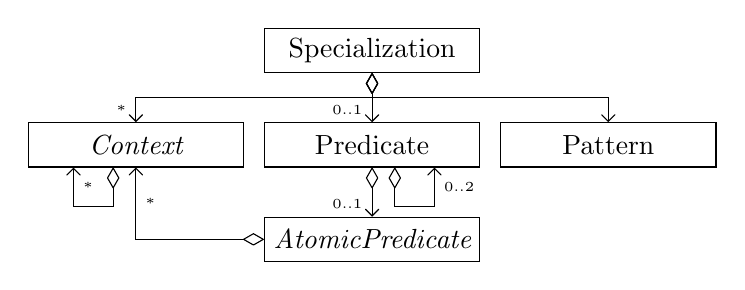
\begin{tikzpicture}[x=30mm,y=12mm]
\tikzset{CODE/.style={draw,chamfered rectangle,chamfered rectangle corners=north east,text centered,minimum height=1.6em}}
\tikzset{CLASSES/.style={draw,rectangle,text centered,minimum height=1.6em}}
\tikzset{CLASS/.style={draw,rectangle,text centered,minimum height=1.6em}}
\tikzset{MULTIPART CLASS/.style={CLASS,rectangle split,rectangle split parts=2}}

\tikzset{EXTENDS/.style={draw,-open triangle 90}}
\tikzset{ASSOCIATES/.style={draw,-angle 90}}
\tikzset{INSTANTIATES/.style={draw,dashed,-angle 90}}
\tikzset{AGGREGATES/.style={draw,open diamond-angle 90}}

\tikzset{CARDINALITY/.style={auto=right,near end,font=\tiny}}

\tikzset{DINGBATS/.style={circle,fill=white,inner sep=-0.5pt}}

\begin{scope}[text width=2.5cm]
\node[CLASS] (specialization) at (0,-1) {\lstinline{Specialization}};
\path (specialization)
  -- +(-1,-1) node[CLASS] (context) {\lstinlineabstract{Context}}
  -- +(+0,-1) node[CLASS] (expression) {\lstinline{Predicate}}
  -- +(+1,-1) node[CLASS] (pattern) {\lstinline{Pattern}};
\path (expression)
  -- +(0,-1) node[CLASS] (atomic predicate) {\lstinlineabstract{AtomicPredicate}};
\end{scope}

\path [AGGREGATES] (specialization) -- +(0,-0.5) -| (pattern);
\path [AGGREGATES] (specialization) -- +(0,-0.5) -| node[CARDINALITY] {*} (context);
\path [AGGREGATES] (specialization) -- +(0,-0.5) -| node[CARDINALITY] {0..1}  (expression);

\path [AGGREGATES] (context.-135) -- ++(0,-5mm) -| node[CARDINALITY] {*} (context.-160);

\path [AGGREGATES] (atomic predicate) -| node[CARDINALITY] {*} (context);

\path [AGGREGATES] (expression) -- node[CARDINALITY] {0..1} (atomic predicate);
\path [AGGREGATES] (expression.-45) -- ++(0,-5mm) -| node[CARDINALITY] {0..2} (expression.-20);

\end{tikzpicture}
\caption{Meta-model of a Specialization in ALIA4J.}
\label{fig:specialization}
\end{figure}

Depending on the definition of the instance pointcut, LIAM models of the underlying pointcuts have to be created in different ways.
For pointcut expressions that are directly provided, we use a library function provided by ALIA4J which takes a String containing an AspectJ pointcut as input.
We have extended this library to also understand the \lstinline{returning} pointcut designator.
All these parts are optional; a missing part can be represented as an empty set of Specializations in LIAM.

\begin{lstlisting}[float,caption={Example of an instance pointcut using composition and type refinement}, label=lst:example:compo:ref,moreemph=instance]
static instance pointcut ${ipc}<${Type}>:
ipc1<${Type2}> || ~\label{lst:example:ip:or}~
before(${pc_add_before}) || after(${pc_add_after}) UNTIL 
before(${pc_remove_before}) || after(${pc_remove_after};
\end{lstlisting}

For the example instance pointcut presented in listing~\ref{lst:example:compo:ref}, we show the code generated for the method creating the LIAM model for the add/before pointcut in listing~\ref{lst:example:compoRefGen}; the other methods are generated analogously.
Line~\ref{lst:example:simple} shows the transformation of an AspectJ pointcut into a set of Specializations in the LIAM meta-model by passing the pointcut as a String---represented by \lstinline!${pc_add_before}! in~\ref{lst:example:compo:ref} and~\ref{lst:example:compoRefGen}---the above mentioned library function.

What is generated from an instance pointcut reference is shown in line~\ref{lst:example:ref}: the LIAM model of the referenced instance pointcut is invoked.
If there is a type refinement defined for this instance pointcut reference, we add a restriction to the retrieved Specializations.
The implementation of the \lstinline!addTypeConstraint! method returns a copy of the passed Specializations where the Predicate is extended with a test that the bound value is an instance of \lstinline!${Type2}! (cf.\ line~\ref{lst:example:restriction}).
Finally, the full LIAM model of the pointcut definition is retrieved by forming the disjunction of the LIAM model for the direct pointcut expression and the LIAM model for the instance-pointcut-reference expression (cf.\ line~\ref{lst:example:composition})---which can itself consist of conjunctions and disjunctions of multiple instance-pointcut references.

\begin{lstlisting}[float,caption={Generated code for creating the LIAM model for the add/before pointcut of the example instance pointcut.},label={lst:example:compoRefGen}]
public static Set<Specialization> ${ipc}_add_before() {
	private static Set<Specialization> ${ipc}_add_before;
	if (${ipc}_add_before == null) {
		Set<Specialization> simpleIPExpr = Util.toSpecializatons("${pc_add_before}", ${Type}); ~\label{lst:example:simple}~
		
		Set<Specialization> ipRefExpr = ipc1_add_before(); ~\label{lst:example:ref}~
		ipRefExpr = Util.addTypeConstraint(ipRefExpr, ${Type2}); ~\label{lst:example:restriction}~
		
		${ipc}_add_before = Util.orSpecializations(ipRefExpr, simpleIPExpr); ~\label{lst:example:composition}~
	}
	return ${ipc}_add_before;
}
\end{lstlisting}

The disjunction performed in line~\ref{lst:example:composition} of listing~\ref{lst:example:compoRefGen} corresponds to the usage of the \lstinline{||} operator in line~\ref{lst:example:ip:or}, listing~\ref{lst:example:compo:ref}.
When the \lstinline{&&} operator is used instead, the method \lstinline{andSpecialization} is used in the generated code, but only in creation of the pointcuts for adding instances to the map. For the removal pointcuts, the simple pointcut expression and the instance pointcut reference expression is always \emph{or}ed.

Finally, the created LIAM models of the pointcuts must be associated with advice invoking the add or remove method for the instance pointcut.
In a LIAM model this is achieved by defining an Attachment, which roughly corresponds to a pointcut-advice pair.
An attachment refers to a set of Specializations, to an \emph{Action}, which specifies the advice functionality, and a \emph{Schedule Information}, which models the time relative to a join point when the action should be executed, i.e., ``before,'' ``after,'' or ``around''.

Listing~\ref{lst:deployment} shows the generated code for creating and deploying the bookkeeping Attachments.
The first Attachment uses the set of Specializations returned by the \lstinline!${ipc}add_before! method (cf.\ line~\ref{lst:deploy:specializations}) and specifies the \lstinline!${ipc}_addInstance! method as action to execute at the selected join points (cf.\ line~\ref{lst:deploy:action}).
As relative execution time, the Attachment uses a ``SystemScheduleInfo''; this is provided by ALIA4J for Attachments performing maintenance whose action should be performed before or after all user actions at a join point, such that all user actions observe the same state of the maintained date.
Thus, when reaching a selected join point the instance is added to the instance pointcut's multiset before (cf.\ line~\ref{lst:deploy:schedule}) any other action can access its current content.
The other Attachments are created analogously.
In the end, all Attachments are deployed through the ALIA4J \lstinline{System}.

\begin{lstlisting}[float,caption={Deployment of the bookkeeping for an instance pointcut.},label=lst:deployment]
public static void ${ipc}_deploy() {
	org.alia4j.fial.System.deploy( ~\label{lst:deploy:deploy}~
		new Attachment(
			${ipc}_add_before(), ~\label{lst:deploy:specializations}~
			createStaticAction(void.class, ${Aspect}.class, "${ipc}_addInstance", new Class[]{${Type}.class}) ~\label{lst:deploy:action}~
			SystemScheduleInfo.BEFORE_FARTHEST), ~\label{lst:deploy:schedule}~
		|Create Attachments for the other three parts analogously.|
		|For the ``after'' parts, use SystemScheduleInfo.AFTER_FARTHEST.|
		|For the ``remove'' parts, specify method ${ipc}_removeInstance.|
		);
}
\end{lstlisting}

To ensure this consistency also between AspectJ advice and our implementation of instance pointcuts, the AspectJ point\-cut-advice definitions must be processed by ALIA4J.
This provides an AspectJ integration which works together with the standard AspectJ tooling.
Using command line arguments the AspectJ compiler can be instructed to omit the weaving phase.
The advice bodies are converted to methods and pointcut expressions are attached to them using Java's annotations which are read by the ALIA4J-AspectJ integration and transformed into Attachments at program start-up.
The code generated by our compiler consists of the above explained methods, as well as plain AspectJ definitions.
When compiling this code with the mentioned command line options, the regular AspectJ pointcut-advice and the behavior of the instance pointcuts are both executed by ALIA4J, thus ensuring a consistent execution order.


\section{Evaluation}








\section{Related Work}
AO-extensions for improving aspect-object relationships are proposed in several studies. Sakurai et al.~\cite{sakurai2004association} proposed Association Aspects. This is an extention to aspect instantiation mechanisms in AspectJ to declaratively associate an aspect to a tuple of objects. In this work the type of object tuples are declared with \lstinline{perobjects} clause and the specific objects are selected by pointcuts. This work offers a method for defining relationships between objects. Similar to association aspects, Relationship Aspects \cite{pearce2006relationship} also offer a declarative mechanism to define relationships between objects, which are cross-cutting to the OO-implementation. This work focuses on managing relationships between associated objects. Bodden et al.~ \cite{bodden2008relational} claim that the previous two lack generality and propose a tracematch-based approach. Although the semantics of the approaches are very similar, Bodden et al.\ combine features of thread safety, memory safety, per-association state and binding of primitive values or values of non-weavable classes. Our approach, also extending AO, differs from these approaches since our aim is not defining new relationships but using the existing structures as a base to group objects together for behavior extensions. Our approach also offers additional features of composition and refinement.

The ``dflow'' pointcut~\cite{kawauchi:aosd-aosdsec04} is an extension to AspectJ that can be used to reason about the values bound by pointcut expressions. Thereby it can be specified that a pointcut only matches at a join point when the origin of the specified value from the context of this join point did or did not appear in the context of another, previous join point (also specified in terms of a pointcut expression). This construct is limited to restricting the applicability of pointcut expressions rather than reifying all objects that match certain criteria, as our approach does.

Another related field is Object Query Languages~(OQL) which are used to query objects in an object-oriented program~\cite{cluet1998designing}. However OQLs do not support event based querying as presented in our approach. It is interesting to combine  OQL like features with instance pointcuts; we will explore this in future work. 


\section{Conclusion and Future Work}
In this work we have presented instance pointcuts, a specialized pointcut mechanism for reifying categories of objects. Our approach provides a declarative syntax for defining events when an object starts or ends to belong to a category. Instance pointcuts maintain multisets providing a count for objects which participate in the same event more than once. Instance pointcut sets can be accessed easily and any changes to this set can also be monitored with the help of automatically created set monitoring pointcuts. The sets can be declaratively composed, which allows reuse of existing instance pointcuts and consistency among corresponding multisets. Finally, we have presented our compilation approach for instance pointcuts based on the generation of LIAM models and plain AspectJ code.

The syntax and expressiveness of instance pointcuts partially depend on the underlying AO language; this is evident especially in our usage of the AspectJ pointcut language in the specification of events. Since AspectJ's join points are ``regions in time'' rather than events, we had to add the ``before'' and `` after'' keywords to our add and remove expressions. Thus, compiling to a different target language with native support for events (e.g., EScala~\cite{Gasiunas2011} or Composition Filters~\cite{Bergmans2001b}, the point-in-time join point model~\cite{masuharafine}) would influence the notation of these expressions.

ALIA4J provided us with the flexibility AspectJ lacked in instance pointcut composition and type refinement. By transforming instance pointcuts to LIAM models, we were able to reuse features offered by ALIA4J and extend some parts of the framework according to our needs. This allowed us to implement a uniform code generator which outputs composable code.


We think the instance pointcut concept is very flexible and can be useful in various applications. It eliminates boilerplate code to a great extent and provides a readable syntax. One relevant field of application for instance pointcuts are design patterns which are known to be good examples for aspect-oriented programming~\cite{hannemann:oopsla02}. Many design patterns exist for defining the behavior for groups of objects; thus implementing them with our instance pointcuts seems to provide a natural benefit. We are currently working on creating object adapters wrapping the objects reified by an instance pointcut.


\bibliographystyle{splncs}
\bibliography{biblio}
\end{document}


%\subsection{Potential Scenarios}
%\begin{enumerate}
	%\item When a product is wish-listed by a GoldCustomer, then apply a discount to it. 
	%\item When products are added to a shopping bag between certain hours, then they are applied the happy-hour discount
	%\item When products are added to GoldCustomer’s shopping bags, apply an additional discount
	%\item When a product is marked low selling by the system, put an advertisement for it on the sidebar → refinement low selling books..., 
	%\item if product is low selling →  notify the vendor
	%\item superset: beauty products, sub-set: beauty products by guerlain which are wishlisted on workdays
	%\item composition:intersect(low selling products && products from Vendor A && products which are lipsticks)
	%\item When it is added to a shopping bag its price may be decreased by applying a discount policy. These examples contain an initial event that is associated with a particular instance, which triggers a follow-up event. 
%\end{enumerate}




